\documentclass[../../thesis.tex]{subfiles}
\graphicspath{{\subfix{diagrams/}}}

\begin{document}
This work aims to reduce the gas amount required for a Uniswap trade by utilizing the properties of zk-rollups. The prototype's goal is to aggregate trade orders of a single trading pair, Ether, and an ERC-20 token of choice. The system is also supposed to remain trustless and not rely on any external data availability to function. By aggregating and offsetting buy and sell orders of a specific pair, the trades will be executed as one, reducing the on-chain gas costs to one trade execution. Correctness of an aggregation batch is ensured by the properties of zkSNARK, allowing for the execution to be verified on-chain. In the proposed design, a Merkle tree with a depth of 16 is used, allowing a maximum of 65536 users in the system. We will now look at the proposed system design and explore the technical implementation after. 

\subsection{Design}
In this section, we will explore the proposed design of the system, looking at the different entities, the functionalities they provide, and the interactions between them. After the high-level design is clear, we will look at the implementation, explaining the system in detail. This system is made up of two entites\footnote{The frontend is omitted here, as it is technically not required for the system to function.} that are required for the system to function: the zkSwap smart-contract and the aggregator.

\begin{figure}[h]
    \centerline{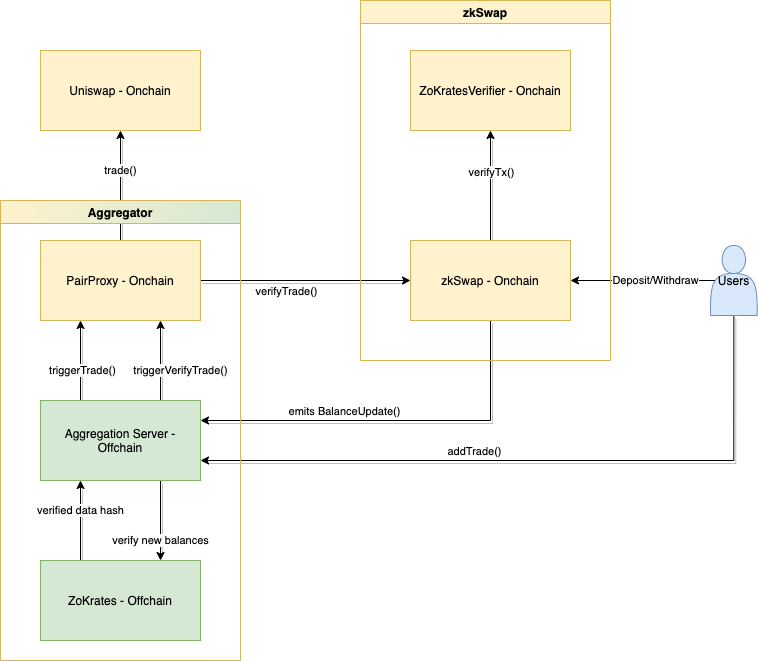
\includegraphics[totalheight=10cm]{diagrams/architecture.png}}
    \caption{High level architecture of zkSwap}
    \label{fig:architecture}
\end{figure}


\subsubsection{zkSwap Smart-Contract}
The zkSwap smart-contract lies at the center of the system. Any state-changing operation is verified by the smart-contract and then finalized by emitting the new state. Assets moving in and out of the system are also processed and stored by the zkSwap smart-contract. We will now look at the different functionalities the zkSwap smart-contract is involved with. 

\paragraph{Deposits}
To use the system, a user first has to deposit funds into the smart-contract. The funds need to be sent as a on-chain transaction to the smart-contract, where they will be stored, while the balance is then represented in layer-2. To deposit funds, a user calls the deposit function in the zkSwap smart-contract and adds the funds to be deposited to the transaction. The deposit details are hashed and stored as a variable, enabling verification of the deposit later. Simultaneously, the user signs the deposit data and sends it to the aggregator as a message. The aggregator aggregates a number of deposits, verifies the correctness in the zkSwap smart-contract, at which point they will show up as balance for the user. This approach of storing funds is also considered non-custodial. As we will explore in the following sections, the funds are secured exclusively by the user's private key. Losing access to that private key results in the funds remaining locked in the smart-contract forever. 

\paragraph{Withdraws}
When withdrawing funds, the user needs to decide between an aggregated withdrawal, similar to the deposit, or an instant on-chain withdrawal. In an aggregated withdraw, a user defines the withdrawal details, signs them and sends them to the aggregator. These are then aggregated, verified in the zkSwap smart-contract, and sent to the users as an on-chain transaction. A user can also withdraw funds by using the instant withdraw feature. While instant withdraws cost significantly more gas, they can be used without the aggregator being online. This protects the user from not being able to withdraw its funds if the aggregator is offline or has turned malicious.

\paragraph{Trades}
When adding a trade order, a user sends the order details to the aggregator. These are then aggregated and executed by the aggregator. Once complete, the funds are sent to the zkSwap smart-contract, were a couple of checks are performed, after which the batch is verified on-chain. This updates the user's balance according to the executed trade.

\paragraph{Verification of Aggregations}
The deposit, withdrawal, and trade features rely on the on-chain verification of a batch, so it makes sense to mention this separately. When aggregating a batch, the aggregator utilizes a zkSNARK circuit that will output a proof object. Each circuit has a corresponding verifier smart-contract that can be used to verify the correctness of the execution by submitting the proof object. When verifying a batch, the zkSwap smart-contract calls the corresponding verifier, checking the proof and thereby the correct aggregation. The new balances are now emitted, finalizing the aggregation.

\subsubsection{Aggregator}
As the name implies, the aggregator's job is aggregating deposits, withdraws, and trades. It facilitates the aggregation of these operations and is built to ensures correct execution while no trust assumptions are made. The aggregator relies on several different systems to function. In this section we will look at the aggregator from a functional perspective, explaining the core functionalities and what systems are relied on.

\paragraph{Deposits and Withdraws}
When a user deposits or withdraws funds, choosing the aggregated type, the user sends a signature of the deposit/withdraw operation to the aggregator. The aggregator receives these messages, collecting them as the next aggregation batch. Once a number of messages have been received, the new balances are calculated and passed to the corresponding zkSNARK circuit, where the correctness of the balances and signature is checked. If this is successful, a zkSNARK proof object is created. The aggregator now sends the proof, along with the new balances, to the zkSwap smart-contract. If the proof is valid, the new balances are emitted by the zkSwap contract. Each withdrawal will now be credited by sending the requested funds to the users. 

\paragraph{Aggregating Trades}
A user can make a trade by sending a message to the aggregator. Similar to deposits and withdraws, the aggregator collects messages as the next aggregation batch. All received trade messages are now aggregated and offset internally, resulting in the net-trade that must be executed to honor all batched trades. The net-trade is then sent to the `PairProxy' smart-contract as an on-chain transaction, which in turn will execute the trade on Uniswap. The details and reasoning of this contract will be explained in the implementation section. Once the trade is executed, the new balances are calculated, and the correctness is ensured by using the corresponding zkSNARK circuit. The resulting proof and the new balances are sent to the PairProxy smart-contract. The previously purchased funds are now added to the transaction, forwarding it to the zkSwap smart-contract. The proof is verified, the new balances emitted, and the aggregator is refunded the amount paid in the 'net-trade'. 

\paragraph{Storing Balances in a Merkle Tree}
The aggregator keeps track of the balances by listening to events emitted by the zkSwap smart-contract. When a new event is emitted, the aggregator either updates or adds the balance to the Merkle tree. Since the events stay on-chain, the Merkle tree can always be rebuilt by querying these events and updating the Merkle tree sequentially. The aggregator provides endpoints where balances and corresponding Merkle paths can be queried. It is important to remember that the balances are public and can be queried by anyone.

\paragraph{PairProxy Smart-Contract}
This smart-contract is controlled by the aggregator and is used to execute trades on Uniswap and forward transactions to the zkSwap smart-contract. The aggregator can use it to hold funds, which makes the transactions cheaper. 

\subsubsection{Client Frontend}
The front-end allows the user to interact with the system, calling the functions while providing necessary data in the background. The front-end also can sync the Merkle tree, containing the systems state, locally. While this puts computational strain on the client, it enables instant withdraws without the aggregator being online. In its current design, the front-end could be hosted as a static file in IPFS \cite{benet2014ipfs}, not relying on any server to function, which closely follows Ethereums unstoppable applications ethos. Deposits, withdrawals, and trades are defined and the necessary messages are sent by the front-end. A user's balance and address are also displayed. 

\subsection{Implementation}
In this section, we will look at the different features in detail, explaining how they function. We will begin by mentioning the technologies used and explain the  mechanism used for updating balances, as it is generally the same throughout the system. After, we will explain the different transaction types, explaining them in detail.

\subsubsection{Technologies Used}
In this implementation, a variety of technologies are applied. The smart-contracts are built with Solidity\footnote{https://docs.soliditylang.org/en/v0.8.3/}, a programming language used for building Ethereum smart-contracts. The functionalities of the aggregator are written entirely in Node\footnote{https://nodejs.org/en/}. The zkSNARK side of the system was built with ZoKrates, a toolchain that includes a domain-specific language (DSL) for creating ZoKrates programs. These programs can be compiled into a zkSNARK circuits, along with the corresponding verifier as a Solidity smart-contract. Throughout this work, ZoKrates program and zkSNARK circuit are used somewhat interchangeably. ZoKrates also includes numerous libraries for standardized operations like hashing. The frontend is built in React\footnote{https://reactjs.org/}, a popular javascript-based frontend framework. The prototype that was built for this project can be found on online\footnote{https://github.com/petscheit/bachelor}.

\subsubsection{Storing and Updating Balances} \label{balances}
Balances are represented as a balance object in our system. This object consists of four fields necessary to represent balances correctly: \textit{ethAmount, tokenAmount, userAddress, nonce}. We want to make balance object updates as cheap as possible while not relying on any external data availability. Essentially, this means that we need to store the balances on-chain. Storing data on-chain is typically very expensive. It is crucial to distinguish between storing data in a smart-contracts runtime and storing data in the event log. Both methods of storage are on-chain, while the event log is significantly cheaper to use. However, a disadvantage of using the event log is that it cannot be accessed from a smart-contracts runtime and must be queried by a client. Using the event log solves the external data availability problem. We can store balances cheaply by emitting the `BalanceUpdate' event without relying on other systems to stay online. A client can query the event log, gather the required data and pass it as parameters to the transaction. However, we now need a mechanism to ensure the passed data is correct.

\paragraph{Merkle Trees}
We can achive this by using a Merkle Tree \cite{szydlo2004merkle}. Merkle trees are a suitable data structure, as the Merkle root represents the entire tree's state in a highly compressed form while proving a leaf's inclusion in the tree can be done in \textit{O(log(N))}. These properties are ideal for our use case. Every balance is stored as a leaf in a Merkle tree, running in layer-2. The Merkle tree is built and kept in sync by subscribing to the 'BalanceUpdate' event emitted by our smart-contract. A balance object can be queried from this tree, receiving the valid Merkle path along with the balance object. The correctness of that data can be proven by recreating the Merkle root stored in the zkSwap smart-contract. By storing the Merkle root in the zkSwap smart-contract, we're committing the entire trees state on the blockchain, preventing unauthorized balance updates. It is essential to understand that balances are only updated by emitting the `BalanceUpdate' event and changing the root accordingly. 

\subsubsection{Aggregating Balance Updates} \label{aggr_balance}
Updating a user's balance is at the core of this system. Deposits result in a balance update, as do trades and withdrawals. Before looking at these in detail, it is important to understand how balance updates can be aggregated, reducing the transaction costs for these operations. Since balances are stored in a Merkle Tree, we can ensure the correctness of a balance by running an inclusion proof. However, running this in a smart-contract is expensive, as much hashing is required. The properties of zkSNARK enable us to run the inclusion proofs off-chain in a ZoKrates program. If the ZoKrates program exits successfully, the zkSNARK proof can be used to verify the correct execution of the inclusion proofs on-chain. This verification gives us equal assurances that the execution was done correctly as executing this on-chain directly. We can run inclusion proof for multiple leaves at the same time while the on-chain verification costs largely stay constant\footnote{There is a certain amount of overhead per leaf, the details of which will be explained in S.4}, resulting in gas savings.

\paragraph{Merkle Inclusion Proofs}
To ensure the correctness of balance updates, we first need to verify that the balance is in the Merkle tree. Doing this one by one is simple. Every balance provides its Merkle path, which it can be hashed with. If the resulting hash matches the current Merkle root stored in the zkSwap smart-contract, we can be assured that the provided balance is included in the tree. At the same time, this enables us to reuse the Merkle path for updating the balance. We can change the balance values after a successful inclusion proof and rehash with the Merkle path. The result is the new Merkle root of the entire tree. Since most hashing is done in ZoKrates programs, looking for a hashing function that can efficiently be executed in a zkSNARK circuit is essential. In this implementation, we will utilize the MiMC \cite{albrecht2016mimc} hashing function, as it can be used in zkSNARK circuits efficiently. The MiMC function is used with the Feistel structure and set up with 220 rounds, which is deemed secure. The Merkle tree is hashed with the MiMC hashing algorithm. 

\paragraph{Chaining Inclusion Proofs} \label{chain_inclusion}
When dealing with multiple balances, the inclusion proof can be done the same way. Every balance provides its Merkle path, the resulting Merkle roots should be the same for each balance. Things become more difficult when also updating the balances. Updating the first balance in the batch now invalidates the Merkle path of all following balances. In order for this to work, the Merkle paths for each balance must be created sequentially and relative to each other. We can chain inclusion proofs by sorting the balances beforehand and generating each Merkle path based on the previous balance changes. The new root of the first balance is the old root of the following balance. This can be chained to an infinite length and results in a constant number of hashes required for each balance update. The last hash to be computed is the new Merkle root, representing all balance updates.


\begin{algorithm}
    \SetKwInOut{Input}{Input}
    \SetKwInOut{Output}{Output}

    \underline{function verifyAndUpdateMerkle}\;
    \Input{oldBalances[], newBalances[], merklePaths[], root}
    \Output{newMerkleRoot}
    \ForEach(){oldBalances}
    {
        assert(computeRoot($oldBalances[i]$, $merklePaths[i]$) == $root$)

        root $\gets$ computeRoot($newBalances[i]$, $merklePaths[i]$)
    }

    return $root$

    \caption{Chained merkle inclusion proofs for verifying and updating balances}
\end{algorithm}

\begin{algorithm}
    \SetKwInOut{Input}{Input}
    \SetKwInOut{Output}{Output}

    \underline{function computeRoot}\;
    \Input{balance, merklePaths[]}
    \Output{root}
    computedHash $\gets MiMC(balance)$

    \ForEach(){merklePath}
    {
        \uIf{$merklePath[i][0] == 0$}{
            computedHash $\gets$ MiMC($computedHash$, $merklePath[i][1]$)\;
        }
        \Else{
            computedHash $\gets$ MiMC($merklePath[i][1]$, $computedHash$)\;
        }
    }
    return $computedHash$
    \caption{Computes merkle root of given parameters}
\end{algorithm}

The Merkle path has a binary as the first element of each hash value. That binary represents if the hash is on the left or the right side of the pair. A cleaner solution is to sort the pairs before hashing and decide the position based on the larger value. Limitations of the number range usable in ZoKrates make this infeasible.

\paragraph{Authorizing Balance Updates}
We still need to ensure the user has authorized a balance update. As balance updates are emitted as events, anyone can access them and compute valid Merkle paths for any balance in our system. The data is public, allowing any user to withdraw any balance. To ensure a user is authorized to update a balance, we need to ensure the user controls the private key belonging to the balance user address. We can ensure this by requesting a signature from the user. However, it must be remembered that this signature must also be verifiable in our ZoKrates program, which cannot utilize the secp256k1 curve used for signing Ethereum transactions efficiently \cite{deml_2019}. For this reason, the Baby JubJub \cite{baylinaeddsa} curve is used in combination with the EdDSA signature scheme, which can be run more efficiently in a ZoKrates program. The user submits a signature containing the current Merkle root and the update message, ensuring three things:

\begin{enumerate}
    \item The user is in controls the balance objects addresses private key
    \item The balance update corresponds to the amount in the update message
    \item By signing the current Merkle root, we make sure that the signature cannot be reused in replay attacks
\end{enumerate}

It is important to note that different programs are used for deposits/ withdraws and trade aggregation. As already mentioned, these programs have several checks that ensure the balance changes correspond to the values specified in the signed update message. These will be explained in the respective sections. 

\paragraph{Creating a EdDSA Signature} \label{signature}
At the time of writing, Metamask\footnote{https://metamask.io/} does not support signing with the EdDSA signature scheme on the Baby JubJub curve. Fortunately, we can derive a Baby JubJub private key from an EcDSA signature and then use the derived key to sign with the EdDSA signature scheme over the Baby JubJub curve. This signature can then be verified efficiently in a zkSNARK circuit. It must also be mentioned that we utilize the MiMC hashing function to hash the message, as it is efficient to run in a zkSNARK circuit.

\paragraph{Reducing On-chain Verification Costs} \label{exec_and_reduce}
All of these checks are performed in a ZoKrates program. At this point, we could return the new balances that we have checked for correctness and verify the proof on-chain. Returning the new balances and other variables would result in high gas costs since every output of a ZoKrates program is part of the proof object, which will add an iteration to the verification logic. For this reason, we create a hash of the return values and only return the hash from the ZoKrates program. The aggregator can compute the same values and pass them to the verify transaction, excluded from the proof object. If the passed data is correct, the hash can be recreated in the smart-contract and should match the output of the proof object. Since we need to recreate this hash for every batch we verify on-chain, we use a hashing function that is cheap on-chain. In our case, this is SHA256. While this optimization adds complexity to our circuits, it effectively reduces the gas required to verify a batch, which is the system's goal.

\subsubsection{Deposits}
When using the system, a user first has to deposit funds. Since the entire idea of zk-rollup is to move funds to layer-2, the deposit function can be seen as a bridge that connects the mainnet and layer-2. When a user makes a deposit, the funds are represented as a balance object in layer-2. The balance object gives custody to these funds. When moving funds in layer-2, the funds residing in the smart-contract are not moved. Instead, the balance objects are updated, representing the movement of funds. Since a balance object gives a user custody of represented funds, it can always be redeemed, moving from layer-2 back to mainnet. 

\paragraph{Movement of Funds}
To move funds to layer-2, a user first needs to send the funds to the zkSwap smart-contract. Funds can be sent by calling the deposit function in the zkSwap smart-contract and attaching the funds to the transaction. To verify the deposits in a later step, we create a recursive deposit hash by hashing the deposited amount, type, and user address with the existing deposit hash. The deposit hash is computed sequentially and ensures users deposited the funds they claimed.

\paragraph{Aggregating Deposits} \label{aggr_deps}
After the funds have been sent to the smart-contract, the user creates a signature containing the type of aggregation (deposit/withdraw), Ether and token balance changes, the user's address, and the current Merkle root. This signature is sent to the aggregator as an HTTP request. The aggregator checks the following: 

\begin{enumerate}
    \item Validity of signature
    \item Merkle root in zkSwap smart-contract matches signed root
    \item Funds were deposited into the zkSwap smart-contract by recreating the deposit hash
\end{enumerate}

These checks are strictly speaking not necessary for a valid aggregation. However, they ensure invalid orders are not added, which would result in the entire aggregation failing. After several deposits have been received, the aggregation is started. The aggregator now generates a `BalanceMovementObject' for each deposit, containing the old balance, the new balance, the Merkle path, and the signature. The `BalanceMovementObjects' are passed to the `ProcessBalanceMovement' ZoKrates program, along with the current Merkle root. As already explained in detail in S. \ref{aggr_balance}, the following is performed for each `BalanceMovementObject' in the ZoKrates program:

\begin{enumerate}
    \item Check if the tree contains the old balance via inclusion proof
    \item Check the validity of the signature
    \item Check if balance change corresponds to the signed values
    \item Check if new balance contains the same address and incremented nonce
    \item Merkle root in zkSwap smart-contract matches signed root
    \item If a withdraw, generate withdraw object\footnote{The details of this will be explained in S. \ref{with}}
    \item If a deposit, compute deposit hash
    \item Compute the new Merkle root
\end{enumerate}

If these steps terminate without an error, we compute the data hash by hashing \textit{newBalances, oldRoot, newRoot, depositHash, withdrawObjects} with the SHA256 algorithm. The data hash is the only output of our ZoKrates program, as it reduces on-chain verification costs as explained in S. \ref{exec_and_reduce}.

\paragraph{Verifying Deposits On-chain} \
Once the ZoKrates program has run successfully, the proof is generated. The aggregator calls the `verfiyBalanceMovement' function in the zkSwap smart-contract and attaches the proof, along with the new balances, the new Merkle root, and the withdraw objects. The zkSwap smart-contract now performs the following steps:

\begin{enumerate}
    \item Compute withdraw hash by hashing withdraw objects
    \item Compute data hash by hashing balances, old root, new root, deposit hash, and withdraw hash
    \item Ensure computed data hash is equal to zkSNARK proof output
    \item Check zkSNARK proof object with verifier smart-contract
    \item Update root stored in smart-contract and reset deposit hash
    \item Emit new balances, and process withdraw objects by sending funds
\end{enumerate}

The attentive reader might have realized that the old root and the deposit hash were not passed as a transaction parameter. Since these values are computed and stored in the smart-contract, we can use them to compute the data hash. While this is more efficient and reduces the amount of gas needed, it also ensures the correct values were used throughout the aggregation. By including the old Merkle root in the data hash, we ensure a proof object cant be used in replay attacks. Once the balances have been emitted, the balance updates are finalized. 

\begin{figure}[h]
    \centerline{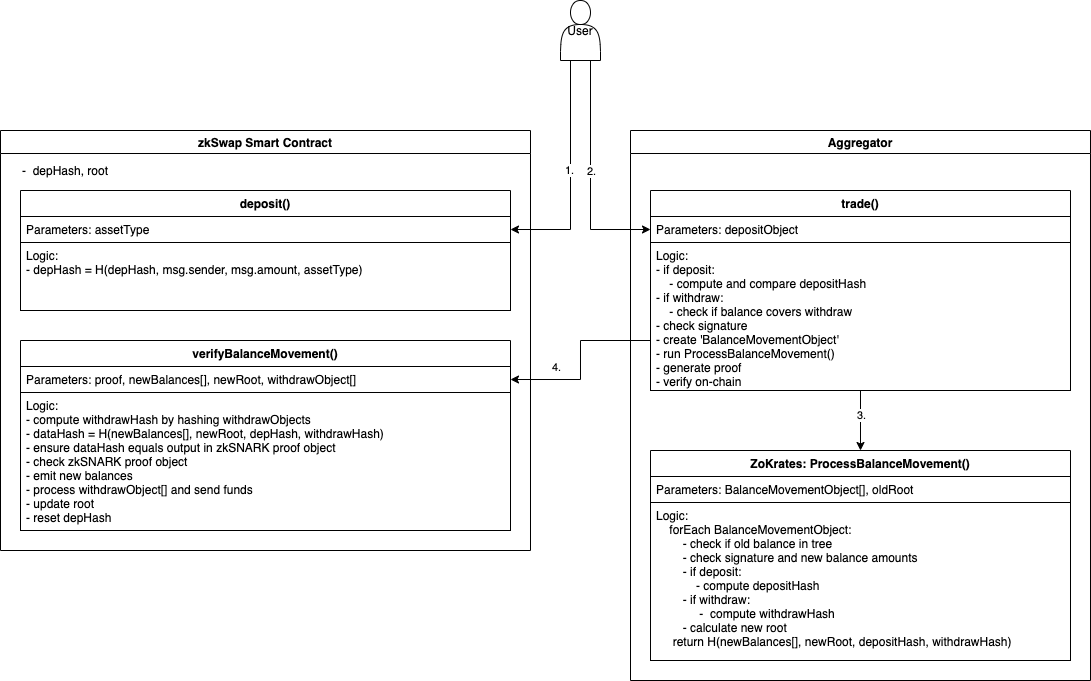
\includegraphics[totalheight=9cm]{diagrams/depositWithdrawAggregated.png}}
    \caption{Interaction diagram of aggregated deposits and withdraws}
    \label{fig:depWithAggr}
\end{figure}

\subsubsection{Withdraws} \label{with}
As briefly mentioned before, withdrawals are batched together with deposits. For this reason, we will only briefly cover the process, as it is largely the same. Instead of sending funds to the zkSwap smart-contract, we are requesting them. As the user already has a balance in the system, an on-chain transaction is not required to trigger a withdrawal. A user creates a signature of its address, the current Merkle root, type of funds, and the amount to be withdrawn and sends it to the aggregator as an HTTP request. Once the aggregation starts, the aggregator checks the users' signatures and ensures that the balance covers the withdrawal. Just like with deposits, a `BalanceMovementObject' is created, the type set to withdraw. The `ProcessBalanceMovement' checks signature, the balances and if the the balance update corresponds to the amount signed by the user. On top of hashing the new balances, a withdraw object is also hashed, containing the type of funds and the amount. When verifying withdraws and the deposits, the withdraw objects will be used to send the funds from the smart-contract to the users. The new balances are emitted and the root updated. 

\begin{figure}[h]
    \centerline{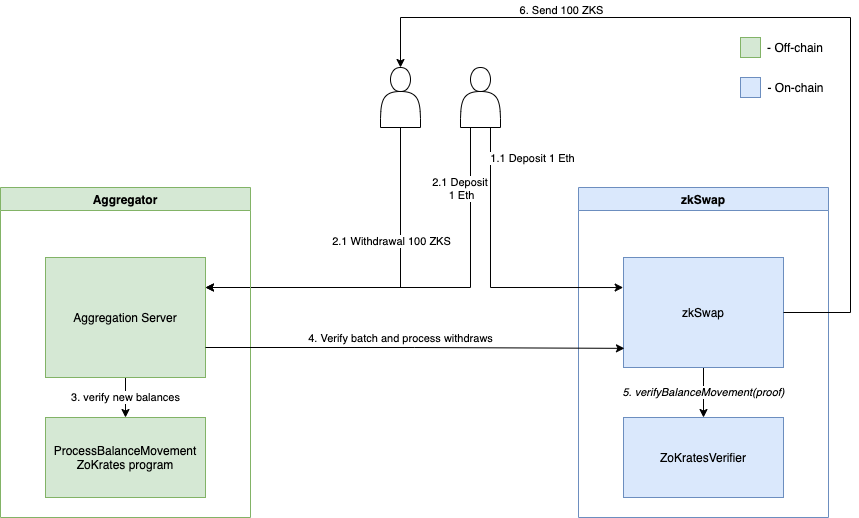
\includegraphics[totalheight=8cm]{diagrams/depWithFlow.png}}
    \caption{Aggregated deposits and withdrawals in detail}
    \label{fig:depWithFlow}
\end{figure}

\subsubsection{Instant Withdraws}
A user also has the option to withdraw instantly without being dependant on the aggregator. Instant withdrawals ensure a user can always withdraw funds, even when the aggregator is failing or offline. Instead of sending the withdrawal request to the aggregator, the withdraw is processed entirely on-chain. The user attaches its balance object, along with the corresponding Merkle path and the withdrawal amount and fund type (Ether/ERC20), to the transaction. As a first step, the Merkle inclusion proof is performed. The balance object is hashed sequentially with the Merkle path. The resulting hash now equals the Merkle root stored in the zkSwap smart-contract if the correct balance object and Merkle path have been submitted. It is checked if the balance can cover the withdraw. If that is the case, the nonce is incremented, the new balance is calculated, and the new balance object hashed again. The new root is now computed by hashing with the Merkle path and updated in the smart-contract. The funds are now sent to the user, and the new balance is emitted. It must be reiterated that this is done completely on-chain and does not require the aggregator to be online. However, the gas costs of this transaction are high, as using the MiMC hashing algorithm is expensive in a smart-contract.

\paragraph{Authorizing Instant Withdraws}
This, however, is an incomplete explanation, as we are not checking if a user is permitted to withdraw funds. As balance objects are emitted as an event, anyone can access them and compute valid Merkle paths for any balance. Not adding an additional check would allow any user to withdraw any balance. To ensure a user is permitted to update a balance object, we need to ensure the user controls the private key belonging to the balance object's user address. Fortunately, we can ensure this by accessing the sender in the transaction object. The Ethereum blockchain ensures a user can make a transaction by requiring the transaction to be signed with the private key of the sender's address. If that signature is valid, it is proven that the user has access to the address's private key, and the transaction can be executed. Thus, the transactions object sender can be trusted to be in control of the corresponding private key. Instead of passing the user's address as part of the balance object, the smart-contract uses the sender of the transaction object. This mechanism suffices as a security check.

\begin{figure}[h]
    \centerline{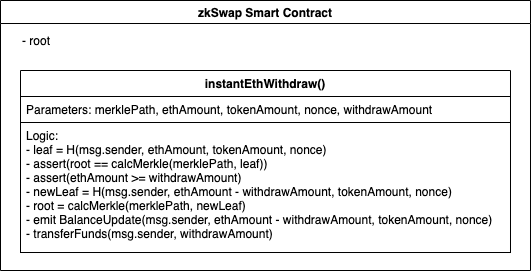
\includegraphics[totalheight=3.7cm]{diagrams/instantWithdraw.png}}
    \caption{Instant withdrawals in detail}
    \label{fig:instWith}
\end{figure}

\subsubsection{Aggregating Trades}
Before explaining the life-cycle of a trade aggregation batch, it makes sense to understand the mechanism that ensures the correct price of trades in an aggregation batch. After, we will go through the entire life-cycle of a batch, starting with a user adding a trade order. 

\paragraph{Ensuring Correct Pricing}
The price between assets is constantly changing. At the same time, trades are being collected for aggregation, which results in a delay between a user sending a trade order and the actual trade execution. During this delay, the price of an asset can change. On top of that, network congestion on the Ethereum blockchain can cause further delays in the execution of a trade. A mechanism is needed to define a worst-case price that is defined before users add orders to the aggregation batch. Once the aggregation is complete, a user can be sure to have paid no worse than the worst-case price.

Another thing to consider is the bid-ask spread that exists in a trading pair. A spread is the difference between the current bid and ask price for an asset, where the bid always has to be a lower price. Intuitively, this makes sense. The spread should at least equal the cost of converting from one asset to the other. Several other factors influence the bid-ask spread for a Uniswap trading pair. In the context of this work, it is sufficient to know that a spread is expected in any trading pair. The bid-ask spread further complicates the mechanism to ensure a worst-case price. 

Buy and sell orders are off-set internally once the aggregation starts, which results in the net-trade. Since we do not know what orders will be received in an aggregation batch, we cannot predict if the net-trade will be a buy or sell order. Since we have a bid-ask spread and can not predict which direction our net-trade will be, we need to define a price range that, at a minimum, equals the current bid-ask spread. An equal price range would suffice to ensure a worst-case price for a net-trade in either direction if executed immediately.
As the aggregation also adds a delay between defining the price range and executing the trade, the price range should be larger than the bid-ask spread. For this reason, the zkSwap smart-contract defines a `minSell' and `maxBuy' price, defining that range. If the price of an asset moves out of the defined range, the trade is not executed and the aggregation canceled. This can be formalized in the following way: 

$$\forall A_o\in A: x_s \leq x_e \leq x_b$$


where:
\begin{description}
\item[$A$] is the current aggregation batch
\item[$A_o$] a trade order
\item[$x_e$] is the effective price 
\item[$x_s$] is the minSell price
\item[$x_b$] is the maxBuy price 
\end{description}

\begin{figure}[h]
    \centerline{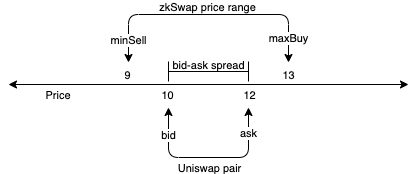
\includegraphics[totalheight=3cm]{diagrams/priceing.png}}
    \caption{Bid-ask spread and zkSwap price range}
    \label{fig:price}
\end{figure}

While this method ensures a worst-case price for a trade, at the same time, a maximum price is defined with it. Since we are matching buy and sell orders in one aggregation, there is no way around this. Once the aggregation is completed and verified on-chain, the new `minSell' and `maxBuy' prices are set based on queried Uniswap prices, which are valid for the next aggregation batch.

\paragraph{Adding an Trade Order}
To make a trade, a user must create a trade object and sign it with its private key. The trade object consists of five fields needed to define the trade: \textit{tradeDirection, deltaEth, deltaToken, userAddress and merkleRoot}. Since ZoKrates only uses unsigned integers, we need the \textit{tradeDirection} to calculate the new balance. Once signed, the trade object is sent to the aggregator as an HTTP request. The aggregator performs the following steps for each incoming trade object:
\begin{enumerate}
    \item Check the signatures validity
    \item Check if users balance covers the trade
    \item Ensures signed merkle root equals the current merkle root\footnote{This prevents orders from being used in malicious replay attacks by the aggregator.}
    \item Checks if implied asset price matches worst-case price
\end{enumerate}

As with deposit and withdrawal aggregation, these checks are only performed to prevent invalid trade orders from being aggregated, as they would result in the cancelation of the entire aggregation batch. Invalid trade are removed from the trade pool. 

\paragraph{Executing Trade and Calculating New Balances}
At some point, the trade aggregation is started. A set block number could trigger this, the number of trade orders received or any other useful condition defined by the aggregator. When aggregation is started, the first step is to calculate the net-trade. Since our system aggregates buy and sell orders, we can offset those internally. By doing this, we can reduce the entire aggregation to one Uniswap trade, which saves gas. At the same time, we are saving on the 0.3\% liquidity provider fee, which is charged based on the trades volume. This trade is now sent as an on-chain transaction to the `PairProxy` contract, where it is executed with Uniswap. The PairProxy contract is explained in detail in S. \ref{pairProxy}. 

The aggregator waits for the PairProxy smart-contract to emit the `TradeComplete' event, which will fire once the trade has been executed, containing the amount of assets acquired in the Uniswap trade. The amount received must at least imply the worth-case price, defined by the zkSwap smart-contract. In most situations, the effective price will be better than the worst-case price. Based on the effective price, the user's post-trade balances are calculated. For each trade, a `BalanceUpdateObject' is created, containing the old balance, the new balance, the Merkle path, and the signed trade object. The `ProcessTrades' ZoKrates program is called, along with the `BalanceUpdateObjects', the current Merkle root, and the worst-case price.

\paragraph{Checking Pricing in ZoKrates}
We want to ensure each trade has the same price, whether it is a buy or sell order. It is also essential that this price is not worse than the worst-case price, defined in the zkSwap smart-contract. We iterate through the `BalanceUpdateObjects', checking if each trade has the same price and making sure it is greater or equal to the worst-case price. While doing this, we also calculate the net-trade, which will represent the flow of funds between the zkSwap smart-contract and the aggregator. After this has been completed, we are assured that each user receives an equal price, at least matching the worst-case price\footnote{The worst-case price will be compared to the one stored in the zkSwap smart-contract at a later stage, enforcing it for the entire aggregation.}, and we have calculated the net-trade, which will be important when finalizing the aggregation.

\paragraph{Verifying Balances and Authorization in ZoKrates}
To ensure the correct aggregation of these trades, we still need to ensure the submitted old balances are part of the Merkle tree and that the user has authorized the trade. While the aggregator has checked this already, it must be remembered that the aggregator is an untrusted party. We need to verify the correct execution of these checks on-chain, which can be achieved with zkSNARK. To ensure this, the following steps are performed for each `BalanceUpdateObject':

\begin{enumerate}
    \item Check if the tree contains old balance via inclusion proof
    \item Check the validity of the signature
    \item Check signed Merkle root equals the current Merkle root
    \item Check balance change is equal or better than signed values\footnote{The signed values will contain the worst-case price. The effective balance change could be better than that.}
    \item Check if new balance contains the same address and incremented nonce
    \item Compute the new Merkle root
\end{enumerate}

These steps largely follow what is described in more detail in S. \ref{aggr_balance}. If these checks pass, we are assured that each balance update was done correctly. The last Merkle root computed in this iteration is the new Merkle root, later updated in the zkSwap smart-contract, and commits the updated state that has been verified here.

\paragraph{Reducing On-chain Verification Costs in ZoKrates}
We have now successfully verified the new balances and could use these values to generate the proof, which will then be used to verify everything on-chain. As explained in S. \ref{exec_and_reduce} we can still reduce the gas needed for verifying the aggregation batch on-chain by hashing the results, thereby removing them from the zkSNARK proof. As the last step of the ZoKrates program, we create the data hash by hashing \textit{newBalances, oldRoot, newRoot, netTrade, worstCasePrice} with the SHA256 algorithm. The data hash is the only output of the ZoKrates program.

\begin{figure}[h]
    \centerline{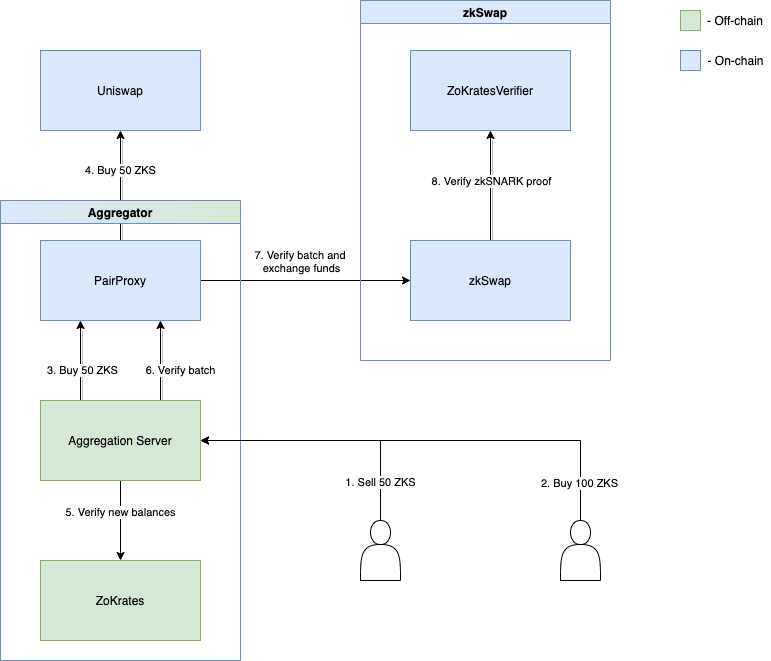
\includegraphics[totalheight=10cm]{diagrams/tradeAggrFlow.png}}
    \caption{Interaction diagram of aggregated trades}
    \label{fig:zokrates}
\end{figure}

\paragraph{Generating Proof and Verifying}
At this point, the aggregator can start the proof generation of the ZoKrates program. To verify the aggregation batch on-chain, the proof object is passed, along with the new balances, the new Merkle root, and the net-trade, and sent to the `PairProxy' smart-contract. The `PairProxy' smart-contract receives the transaction, adds the funds previously traded with Uniswap to the transaction, and forwards it to the `verifyTrades' function in the zkSwap smart-contract, where all following steps are performed. 

\paragraph{Recreating the Data Hash}
As a first step, we recreate the data hash previously computed in the ZoKrates program. By recreating this hash, we ensure the aggregator has performed several steps correctly:

\begin{enumerate}
    \item The balances and new root passed by the aggregator were verified in the ZoKrates program
    \item The net-trade corresponds to the net change of balances
    \item The correct worst-case price was used throughout the aggregation
    \item The current Merkle root equals the old Merkle root in the aggregation, preventing proofs from being used in replay attacks
\end{enumerate}

The worst-case price and old Merkle root are not passed as parameters and are stored in the smart-contract. Including these values in the data hash ensures the aggregator used the correct values when the aggregation batch was started. By including the balances, new root, and net-trade, we ensure the aggregator passes the correct values after the aggregation. The method saves gas in the on-chain verification step and ensures the aggregator executed its tasks correctly. If the hashed value does not equal the output of the proof object, some values were incorrect, resulting in the entire aggregation being canceled. 

\paragraph{Verifying the ZoKrates Proof}
The next thing to be checked is the validity of the zkSNARK proof object. The zkSwap smart-contract can access a verifier contract that was explicitly deployed for this purpose. The `verifyTx()' function is called, and the proof object is passed as a parameter. If the verifier returns true, we have proven that our data hash was computed by running the `ProcessTrades' ZoKrates program. By having proven knowledge of the preimage, the properties of the data hash are extended to the preimage\footnote{Given that SHA256 is assumed to be collision resistant}. At this point, we have proven that the balances were updated correctly.

\paragraph{Exchanging Traded Funds}
Now the funds traded on Uniswap must be exchanged between the aggregator and zkSwap smart-contract. We check if the funds attached to the transaction are equal to the amount specified in the net-trade. It is important to remember that we have checked the correctness of the net-trade by recreating the data hash already. The exchange of funds always needs to result in a solvent zkSwap smart-contract\footnote{The zkSwap contract is solvent if it is always able to cover the withdraw of all balances. The zkSwap contract should always be solvent.}. If the aggregator has attached the correct amount of funds, the zkSwap smart-contract now refunds the aggregator by sending the funds it spent for the Uniswap trade. If an incorrect amount was attached, the aggregation is canceled.

\paragraph{Updating Root and Emitting Balances}
In the last step, we update several variables that are needed in the next batch. The Merkle root stored in the smart-contract must be updated. By recreating the data hash, we have proven the new Merkle root to be correct, so we update it accordingly. The worst-case price also needs to be updated, which can be achieved by querying the current price from Uniswap. The new balances are emitted as `BalanceUpdate' events to finalize the aggregation batch, resulting in the balances being updated for the users, representing the trade. The lifecycle of a trade aggregation is now complete, and the next batch starts.

\begin{figure}[h]
    \centerline{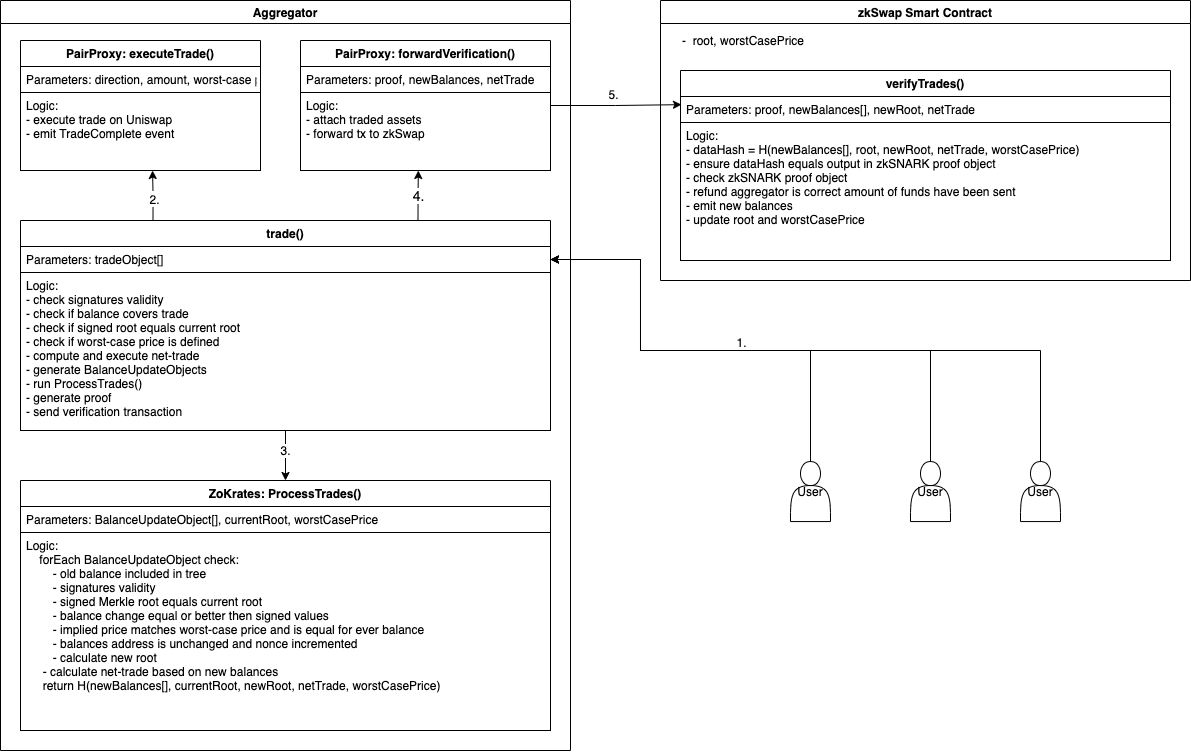
\includegraphics[totalheight=8cm]{diagrams/tradeAggregated.png}}
    \caption{Aggregated trades in detail}
    \label{fig:trade_aggr}
\end{figure}

\subsubsection{PairProxy Smart Contract} \label{pairProxy}
Before explaining the functionalities of this smart-contract, it is essential to understand why it is required for the system to function. There are two reasons: a quirk in the way Ethereum handles return values and the result of dealing with changing price data.
When performing a trade on Uniswap, a user is asked to define a slippage\footnote{Slippage is the difference of the expected and executed price of a trade} for the trade. Since network congestion and the current gas price influence when a transaction is executed, it is necessary to ensure users can set a worst-case price. For this reason, when sending a transaction to the Uniswap trade function, the `minAmountReceived' parameter must be passed, which we provide by using our worst-case price, explained in a previous section. When calling the trade function, the actual amount received is returned as the function's return value. Since this amount might be larger than the amount passed as `minAmountReceived', we need it to calculate the post-trade balances\footnote{The trade also throw an error when the `minAmountReceived' amount cannot be fulfilled. In this case, the aggregator cancels the aggregation}. 

However, a quirk in Ethereums way of handling return values makes this more difficult. A smart-contracts function's return value can only be accessed when called by another smart-contract function. If calling a function as a normal transaction, as the aggregator does, we receive the transaction recipe instead of receiving the function's return value, which does not contain the return value. For this reason, we need the PairProxy smart-contract, which receives transactions, forwards them to the respective smart-contract, emitting the return value as an event, which the transactor can consume. 

The PairProxy smart-contract is used for forwarding transactions to the Uniswap or the zkSwap contracts. After the aggregator has calculated the net-trade, it calls the trade function in the PairProxy contract, passing the calculated trade parameters. The PairProxy contract now calls Uniswaps trade function, receiving funds and the amount as a return value. As it has access to the return value, it emits the `TradeComplete' event, containing the amount received in the trade. As it would be inefficient to send the funds back to the aggregator, they reside in the smart-contract. Since the aggregator is set as the owner of the contract, the funds are stored securely.

When verifying the aggregated trades in the zkSwap smart-contract, the transactions are forwarded by the PairProxy again. Since the funds previously traded still reside in the smart-contract, they are attached to the transaction when forwarded to the zkSwap smart-contract.

\subsection{Limitiations of Current Implementation}
The working implementation of this system is different from the proposed design in certain areas. The differences are mainly the result of two factors: MetaMask not supporting EdDSA natively and being unable to create matching MiMC hashes in ZoKrates and Solidity. The necessary ZoKrates programs have been built and used in the results section but are not integrated into the prototype for the reasons stated above. 

\paragraph{Signatures}
As described in S. \ref{signature}, the authorization of an order or deposit entirely relies on a user signing the trade order and Merkle root. This signature needs to be checked in a ZoKrates program, limiting us to use the EdDSA scheme with the BN128 curve. Hermez \cite{hermez_docs}, a zk-rollup based asset transfer system, has solved this by creating a Baby JubJub\cite{baylinaeddsa} private key from a signed EcDSA message, which can be requested by Metamask. The generated private key can then be used to sign in EdDSA on the BN128 curve. I do not have a written source for this but talked to their team members, who explained how they do this. Since their system is running on the mainnet now, it can be assumed to work. In the system's current form, signatures are not checked at all.

\paragraph{Updating Balances According to Effective Price}
After the aggregator has executed the net-trade on Uniswap, the new balances are calculated based on the worst-case price instead of the effective price the aggregator has paid. Currently, there is no mechanism in place that can ensure this. The aggregator could always claim the worst possible price has been paid (depending on net-trade direction), while keeping the difference for itself. This will be addressed in the open problems section.

\paragraph{Hashing Function}
In its current form, the system does not utilize the MiMC hashing yet. All hashing is currently done with SHA256, limiting the number of trades or deposits/withdraws that can realistically be included in a batch due to the circuit size. The benchmarking results where generated with circuits that utilize MiMC hashes, however, the inability to create matching hashes in Solidity prevents the utilization of the ZoKrates program in the prototype. 

\paragraph{Aggregating Deposits and Withdraws}
Since the MiMC hashes are not implemented yet, the aggregated withdraws are not ether. The necessary ZoKrates programs have been developed, however, due to the inablility to create matching MiMC hashes where never used. In its current form, deposits and withdraws are done on-chain, pretty much the way the instant withdraw works, but using SHA256 to hash the Merkle tree.

\end{document}